%% ----------------------------------------------------------------
%% PreviousWork.tex
%% ---------------------------------------------------------------- 
\chapter{Previous Work} 
\label{Chapter:Previous Work}
\section{Academic Work} 
\label{Section:Academic Work}
A \gls{MLE} is the overall system used by an educational establishment to facilitate and manage learning. This will be comprised of several subsystems (as seen in \autoref{Figure: MLE}).

\begin{figure}[h]
	\centering 
		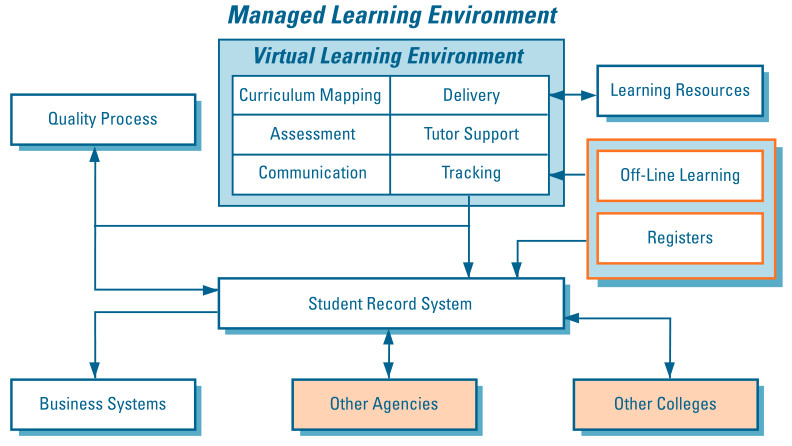
\includegraphics[scale=0.4]{../figures/MLE.png} 		
	\caption{\label{Figure: MLE} Components of an \gls{MLE} \citep{mle}} 	
\end{figure}

This project focuses on the Assessment system in the \gls{VLE}.

\subsection{eAssessment}
An \gls{eAssessment} (also known as \gls{CAidA}, \gls{CAssA}, \gls{CBA}) is the process of making, viewing and scoring assessments using a computer. In this report these processes will be carried out by several tools - the ``\gls{authoring}" will be responsible for creating the questions and assembling the test and the ``\gls{delivery}" will be responsible for displaying and scoring the assessments. These tools must be interoperable, meaning they must use data formats that are compatible with each other.

This project focuses on the use of quizzes and polls within videos as a means of assessment.

\subsubsection{Quiz Definition Standards}
\label{Subsubsection:Quiz Definition Standards}
In order to store and display the questions in an \gls{eAssessment}, a schema for the questions must be defined. The only formally defined standard found was IMS Global's \gls{qti} specification\footnote{\url{http://www.imsglobal.org/question/\#version2.1} Last Accessed: 24 Nov 14}. Some other quiz (wiki-like) definitions were found including Moodle's General Import Format Technology (GIFT)\footnote{\url{https://docs.moodle.org/28/en/GIFT_format} Last Accessed: 24 Nov 14} and Aiken formats\footnote{\url{https://docs.moodle.org/23/en/Aiken_format} Last Accessed: 24 Nov 14}.

GIFT is a question mark up by Moodle\footnote{\url{https://moodle.org} Last Accessed: 24 Nov 14}. It allows users to use a text editor to create questions in some simple formats. There is a strict compliance to specific syntax required and for complex questions it is no longer intuitive \citep{failQTI}. Aiken is another mark up that is designed to be more easily human-readable, again it has strict syntax that must be adhered to or the imports to Moodle would fail.

\gls{qti} is an interoperability standard for eAssessments. The specification overview \citep{qtiOverview} splits the \gls{eAssessment} system into five systems: authoring tool, item bank, test construction tool, assessment delivery system and learning system (see \autoref{Figure: QTI components}).

\begin{figure}[h]
	\centering 
		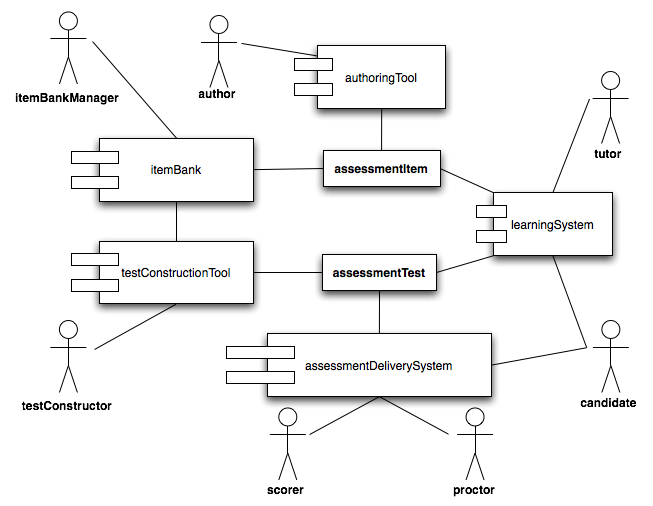
\includegraphics[scale=0.3]{../figures/componentsQTI.png} 		
	\caption{\label{Figure: QTI components} QTI components diagram \citep{qtiOverview}} 	
\end{figure}

In the \gls{qti} definition the authoring tool is used to create individual questions. However many systems combine this with the Item Bank and Test Construction Tool. For this report ``\gls{authoring}" refers to this combination and, as such, an authoring tool is used to create whole quizzes.

\cite{wikieassessment} state:
\begin{quote}
The major promise of QTI is that by introduction of common format developers can concentrate on developing innovative tools, whereas teachers can focus on defining new and groundbreaking methods of how to apply those tools in an online environment.
\end{quote}

It is a very complex specification with many ambiguous or optional elements. The complexity of the specification increases the likelihood for errors in the implementation as it opens up opportunities for developers to interpret the specification in different ways \citep{failQTI}. This means the intent of the original author may be lost.

\gls{qti} v2.1 was finalised in 2012 \citep{qtiOverview} but up to this point the standard was not widely used \citep{eps265979} as there were several fundamental flaws in the standard. When the v2.1 draft was withdrawn in 2009 Rib Abel (IMS GLC CEO) was quoted as saying (on v2.0) ``it’s deficiencies are well known and IMS does not recommend implementation of it [\dots] the only version of QTI that is fully endorsed by IMS GLC is v1.2.1"\footnote{\url{http://lists.ucles.org.uk/public/ims-qti/2009-March/001463.html}}. This standard gave definitions in natural language. These could often be long-winded and ambiguous, making the standard difficult to implement\citep{failQTI, Sclater2007}.

\gls{qti} v2.1 defines 18 types of interaction (question, answers and response patterns) \citep{qtiImplementation}:
\begin{multicols}{3}
\begin{enumerate}
\item Choice
\item Order
\item Associate
\item Match
\item Gap match
\item Inline choice
\item Text entry
\item Extended text
\item Hot text
\item Hotspot
\item Select point
\item Graphic order
\item Graphic associate
\item Graphic gap match
\item Position object
\item Slider
\item Drawing
\item Upload file
\end{enumerate}
\end{multicols}

In addition, assessment items can have template and/or adaptive behaviour giving 72 options for each item's type. 

Template items have variables in the questions and answers. These are set as the question is viewed. This allows similar questions to be defined using the same assessment item (e.g. changing the numbers in a maths problem).

Adaptive items are scored over a series of questions. Different questions are displayed based on the answer given for the previous question(s) in the sequence. This branching behaviour is defined by setting the \lstinline!adaptive! attribute to true. 

\subsubsection{Usage of Video in eAssessment}
\label{Subsubsection:Usage of Video in eAssessment}
Video is often used as a medium to convey educational material as it appeals to different learning styles. When video is streamed there is a lack of interactivity and user control \citep{eps267281}. To involve the user more, interactive elements must be added. \cite{eps267281} found that 75\% of users agreed or strongly agreed that interactive video had enhanced their learning experience but at the time of the paper there was no evidence of interactive video being used as a learning tool.

By adding polls and quizzes into videos immediate meaningful feedback can easily be given, a key feature of formative assessment \citep{eps265979}. Having the questions integrated into the video allows the appropriate sections to be automatically re-watched. 
\subsubsection{Accessibility and Usability}
\label{Subsubsection:Accessibility and Usability}
To allow interoperability between the \gls{eAssessment} systems the \gls{qti} specification involves both the model and the view of the data \citep{wikieassessment} making accessibility difficult to add in later. This means many systems that comply with the \gls{qti} specification are inaccessible. Moodle, for example, uses a video player to display content that is completely inaccessible to a user only using a keyboard\footnote{\url{https://tracker.moodle.org/browse/MDL-36081} Last Accessed: 24 Nov 14}.

\gls{eAssessment} systems require an authoring tool that is easily understood by people who do not have an in depth technical knowledge (e.g. teachers). Often authoring tools that implement the \gls{qti} standard are too technical for this \citep{wikieassessment}. These tools need to improve their accessibility and usability, keeping the time commitments for users reasonable \citep{eps271236, eps265979} or they will not be used.

There are many ways of conveying content in a video and none of the methods alone will generally convey the whole message. Most video searches stay on a whole resource level as there is a lack of semantic interlinking \citep{eps273063}. Annotation systems such as Synote\footnote{\url{http://synote.org/synote/} Last Accessed: 24 Nov 14} aim to make videos accessible by adding transcripts and other annotations to them. The videos being annotated may not be owned by the annotator.

\subsubsection{Analytics}
\label{Subsubsection:Analytics}



\newif\ifnote
\notefalse
\ifnote
In \cite{eps265979}:
R2Q2 (deprecated - replaced by QTI Engine)
Constructr - constructr.qtitools.org - proof-of-concept
Playr - playr.qtitools.org - deprecated - effectively our overlays
\fi

\section{Industrial Work} 
\label{Section:Industrial Work}
